\section{}\label{sec:hardware_images}
\FloatBarrier
\begin{figure}[h!]
    \centering
    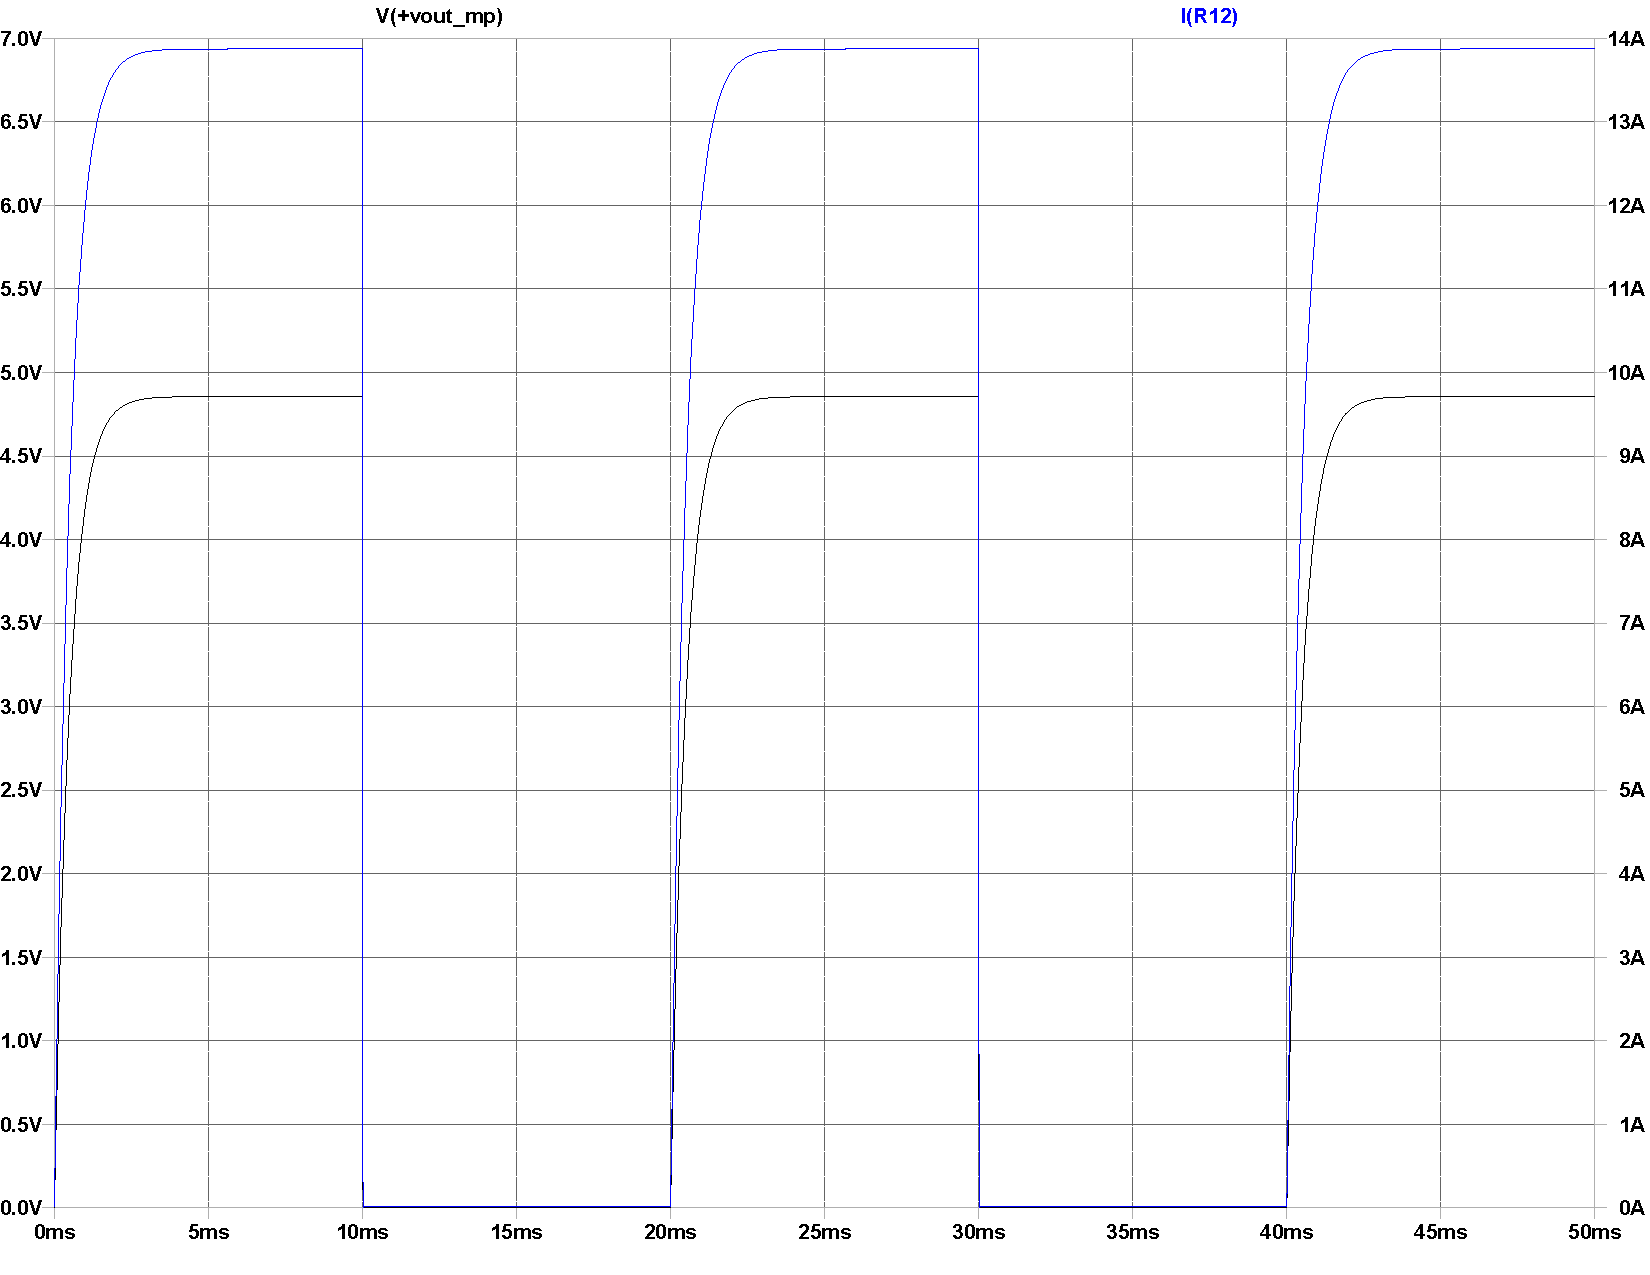
\includegraphics[scale=0.3]{LT3080-1_Transient-response.pdf}
    \caption{12 A linear regulator transient response.}
    \label{fig:LT3080-1_Transient-response}
\end{figure}

\begin{figure}[h!]
    \centering
    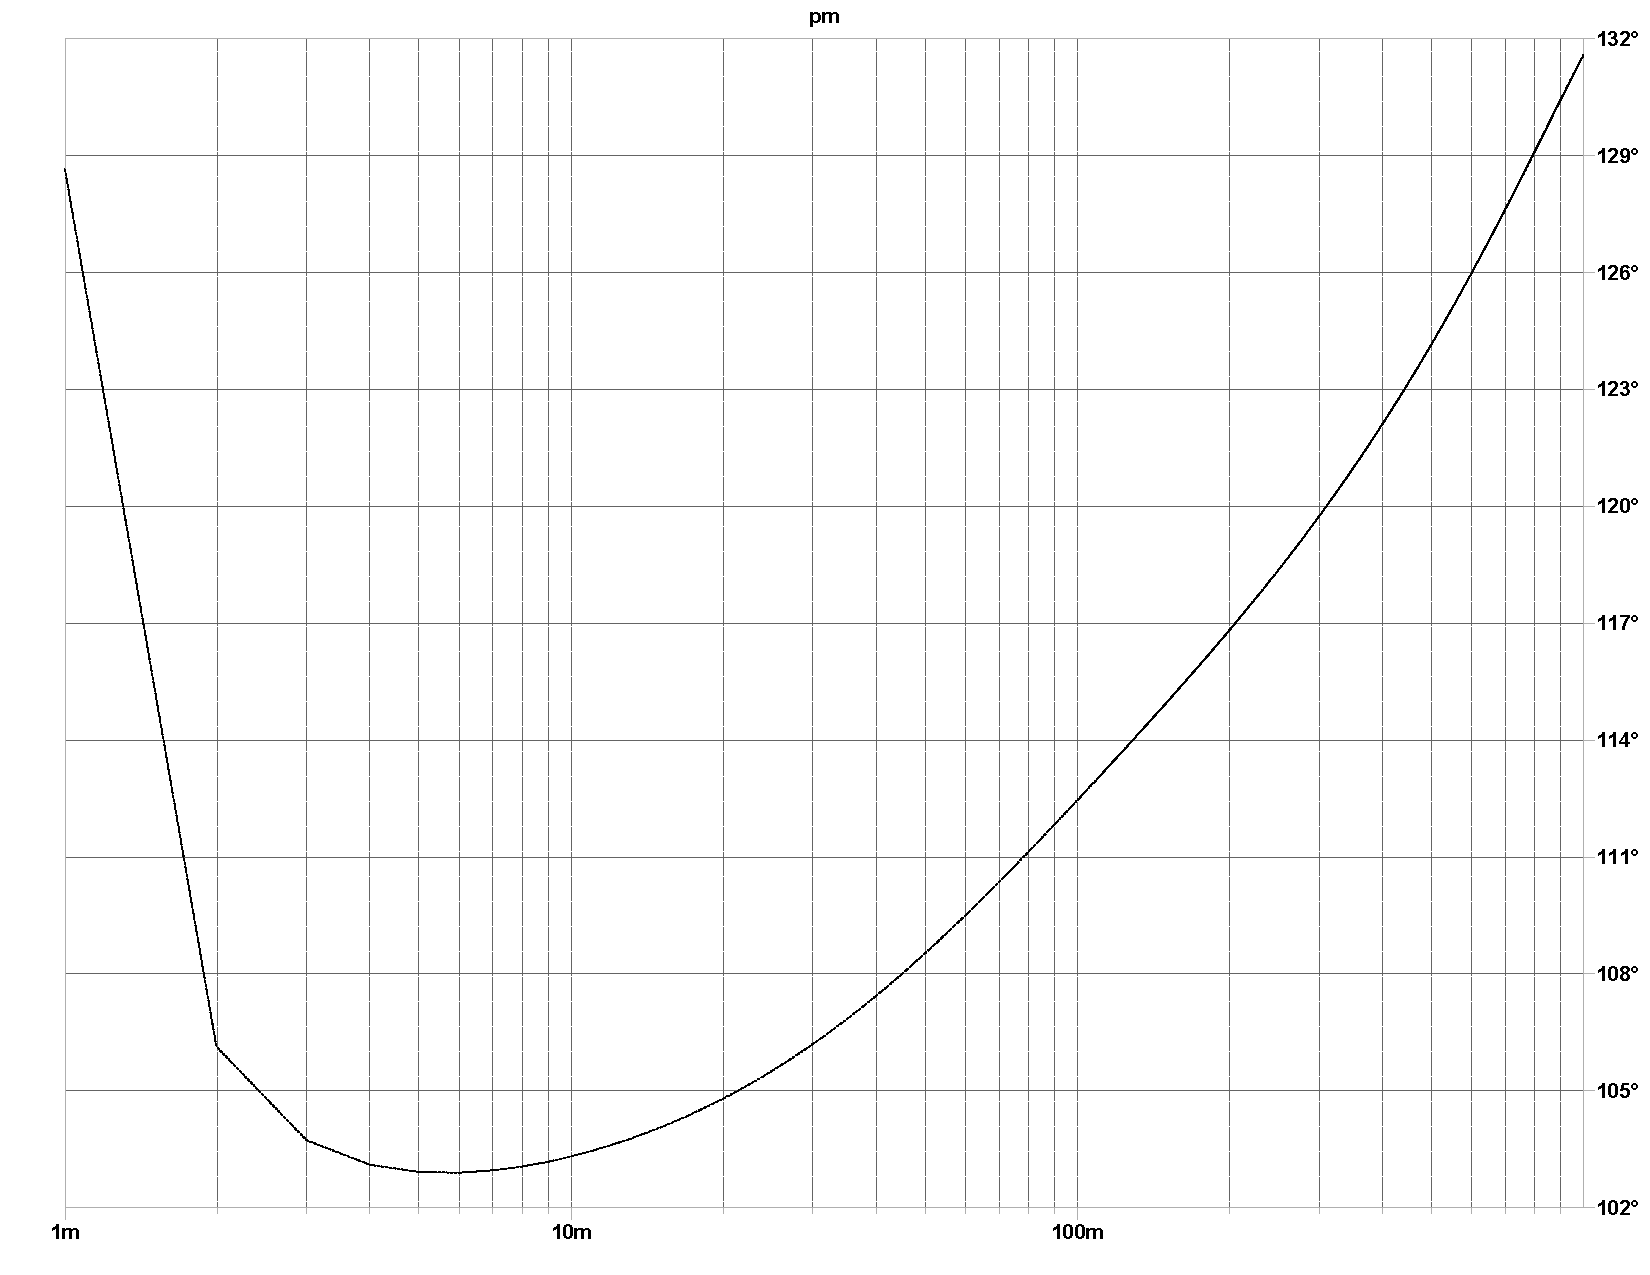
\includegraphics[scale=0.3]{LT3080-1_Phase-margin_VS_setpoint.pdf}
    \caption{12 A linear regulator phase margin vs setpoint (current).}
    \label{fig:LT3080-1_Phase-margin_VS_setpoint}
\end{figure}

\begin{figure}[h!]
    \centering
    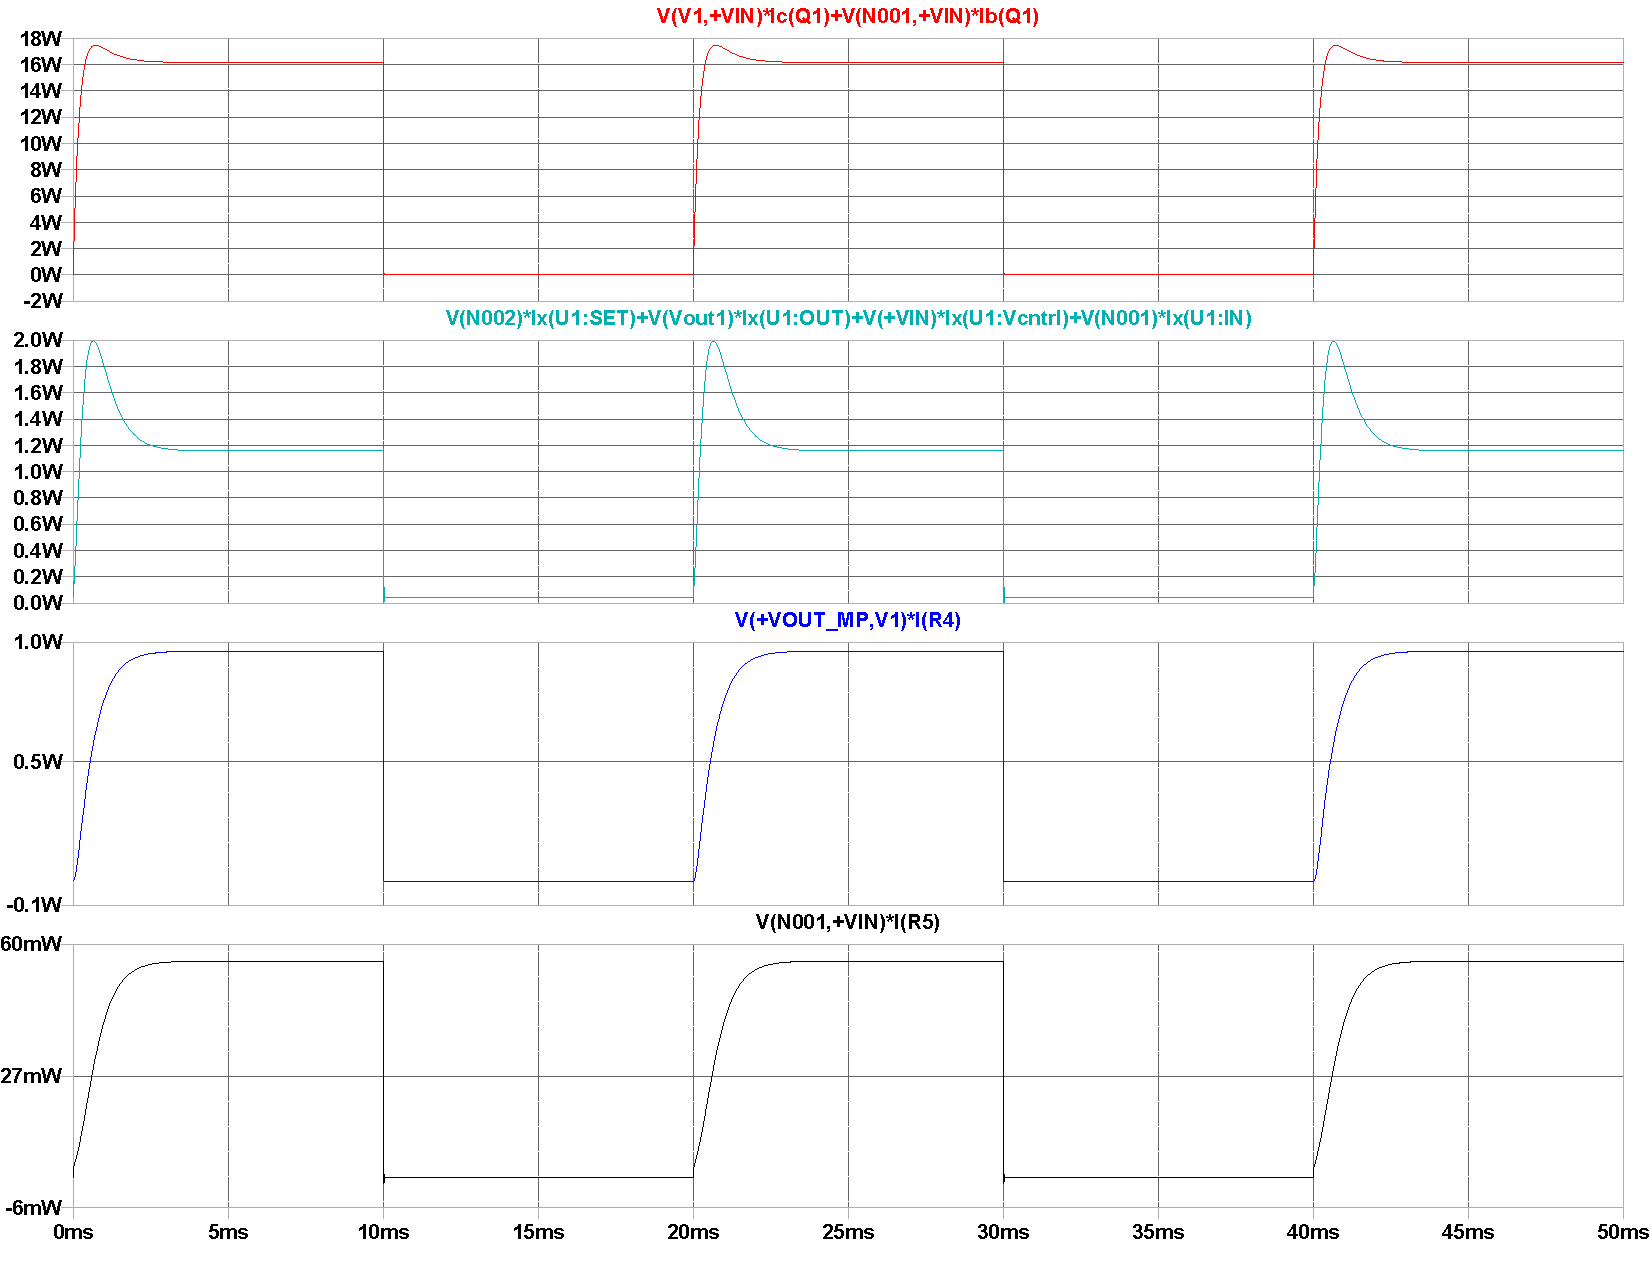
\includegraphics[scale=0.3]{LT3080-1_PowerDissipation.pdf}
    \caption{12 A linear regulator power dissipation.}
    \label{fig:LT3080-1_PowerDissipation}
\end{figure}

\begin{figure}[h!]
    \centering
    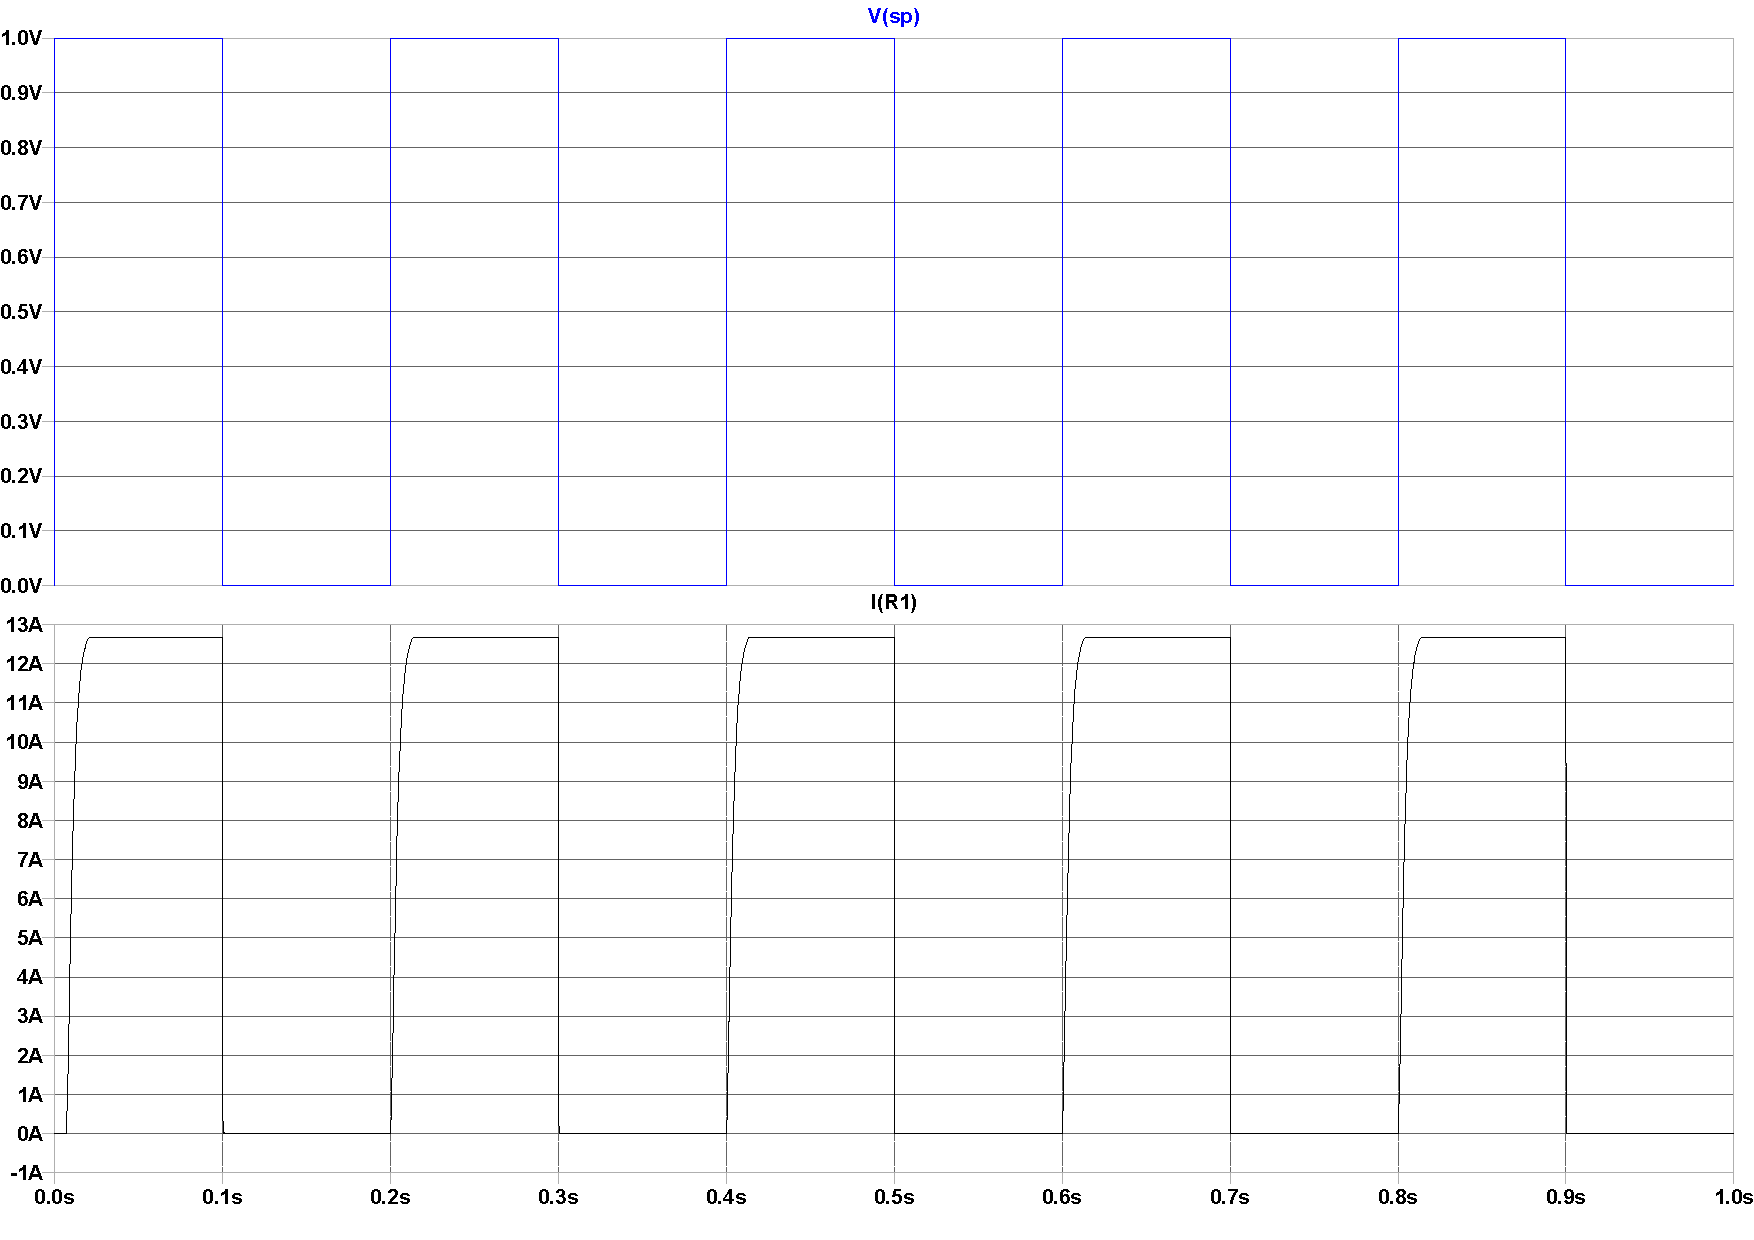
\includegraphics[scale=0.3]{CurrentSinkTransient.pdf}
    \caption{12 A current sink transient responce.}
    \label{fig:CurrentSinkTransient}
\end{figure}

\begin{figure}[h!]
    \centering
    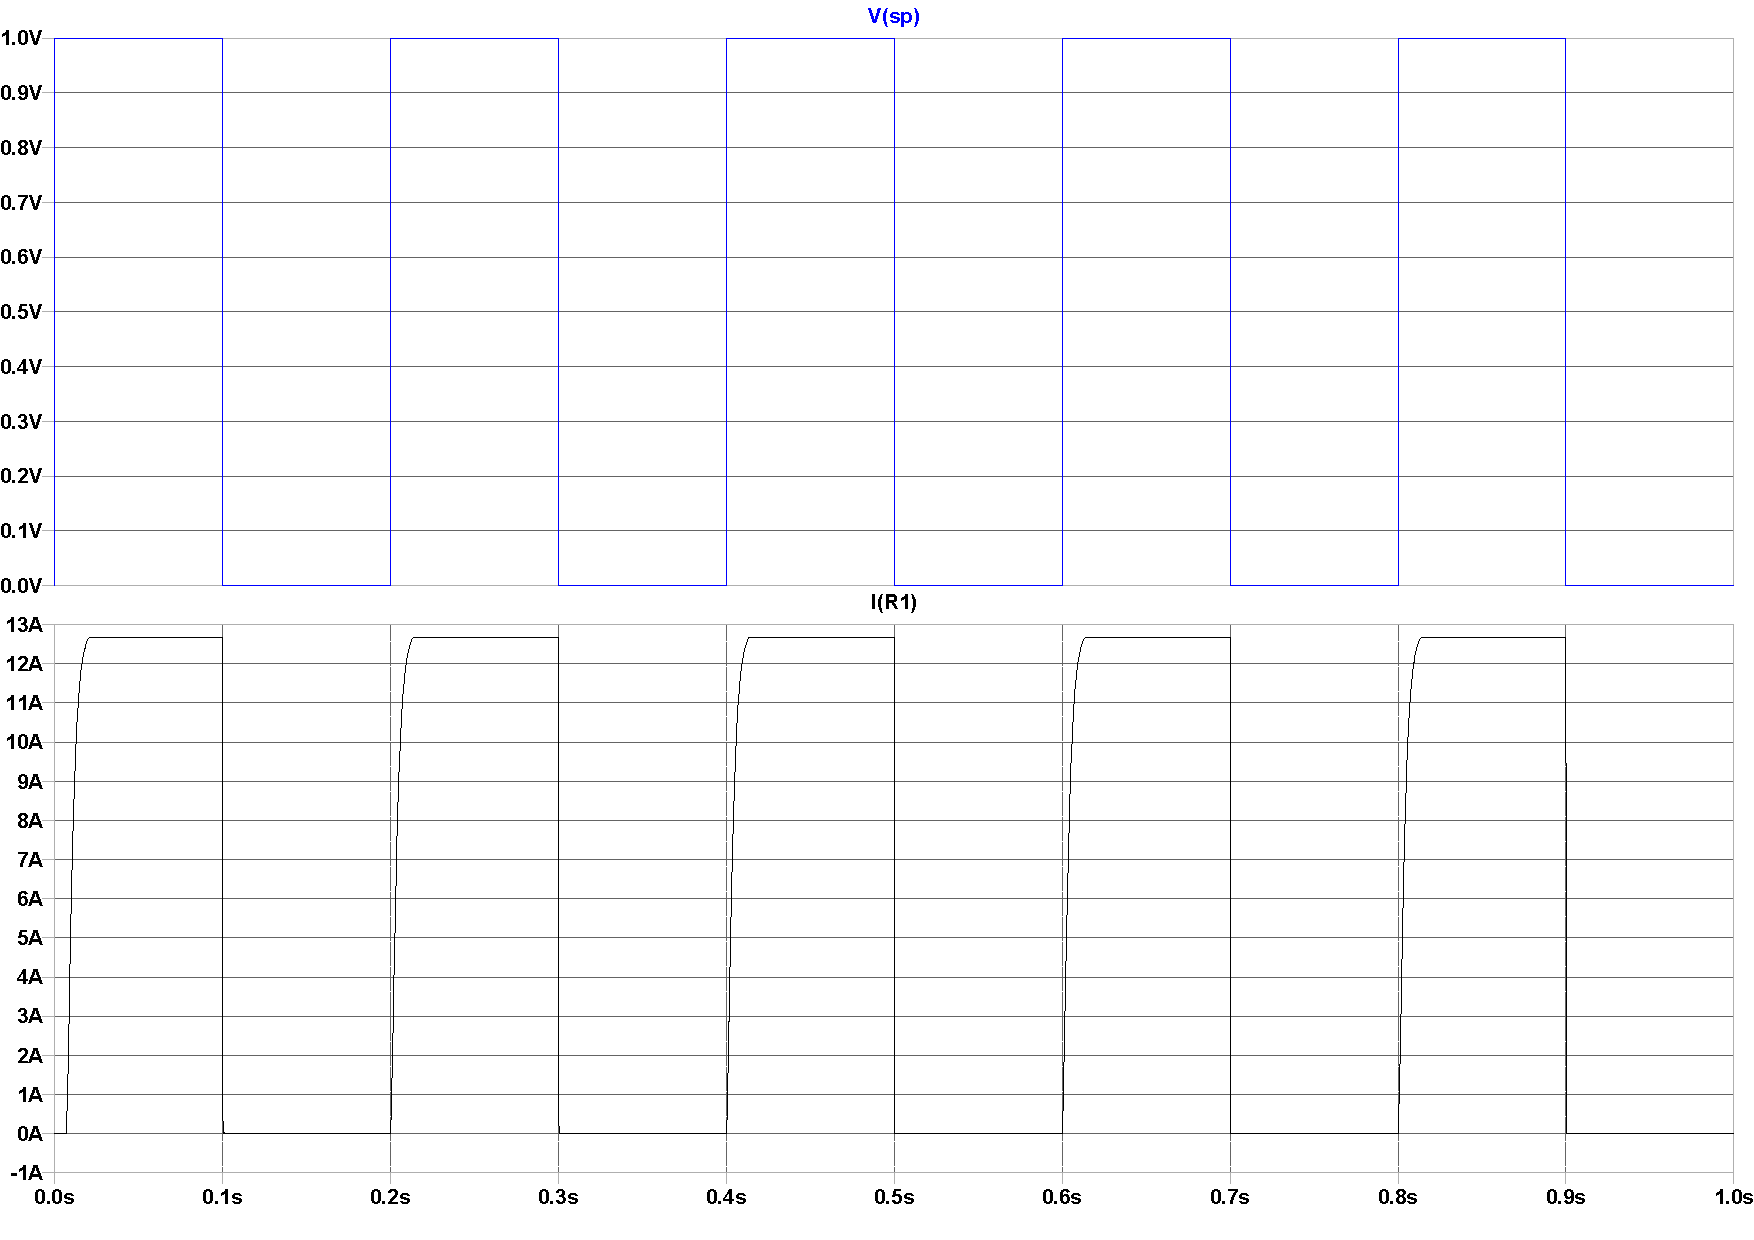
\includegraphics[scale=0.3]{CurrentSinkTransient.pdf}
    \caption{12 A current sink transient responce.}
    \label{fig:CurrentSinkTransient}
\end{figure}

\begin{figure}[h!]
    \centering
    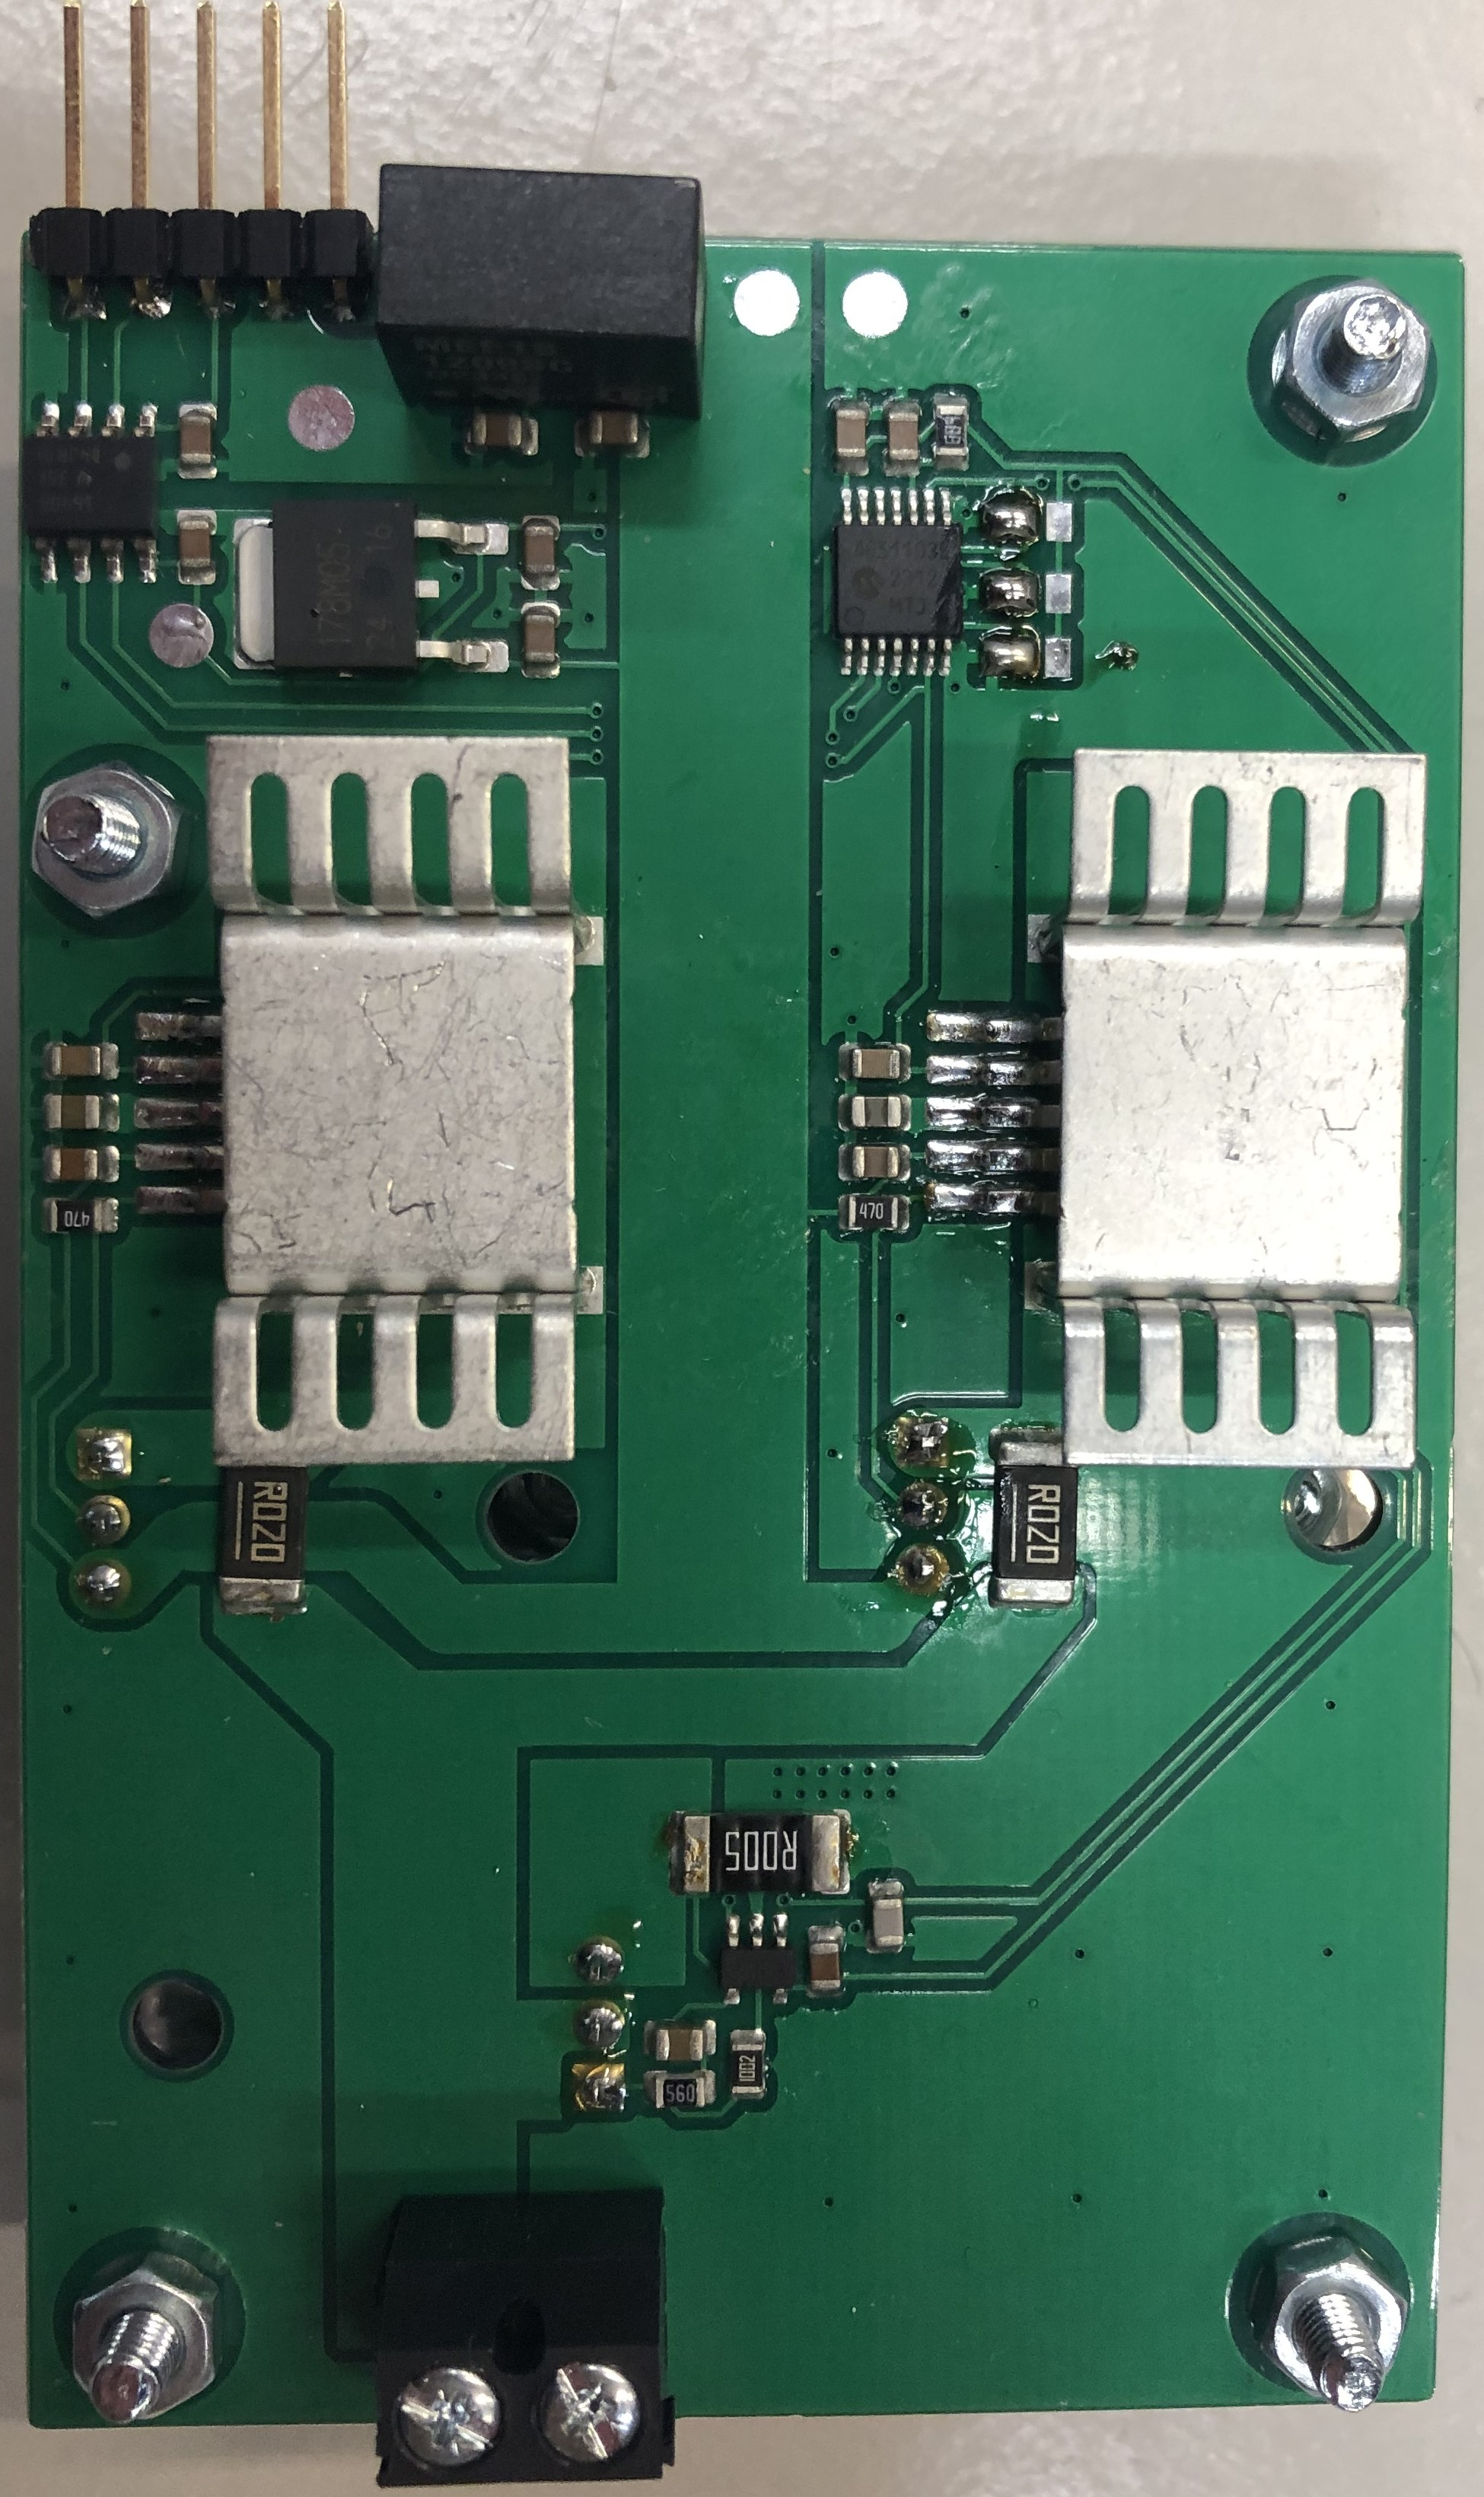
\includegraphics[scale=0.2]{CellBoardTop.jpg}
    \caption{Top view of cell board.}
    \label{fig:CellBoardTop}
\end{figure}

\begin{figure}[h!]
    \centering
    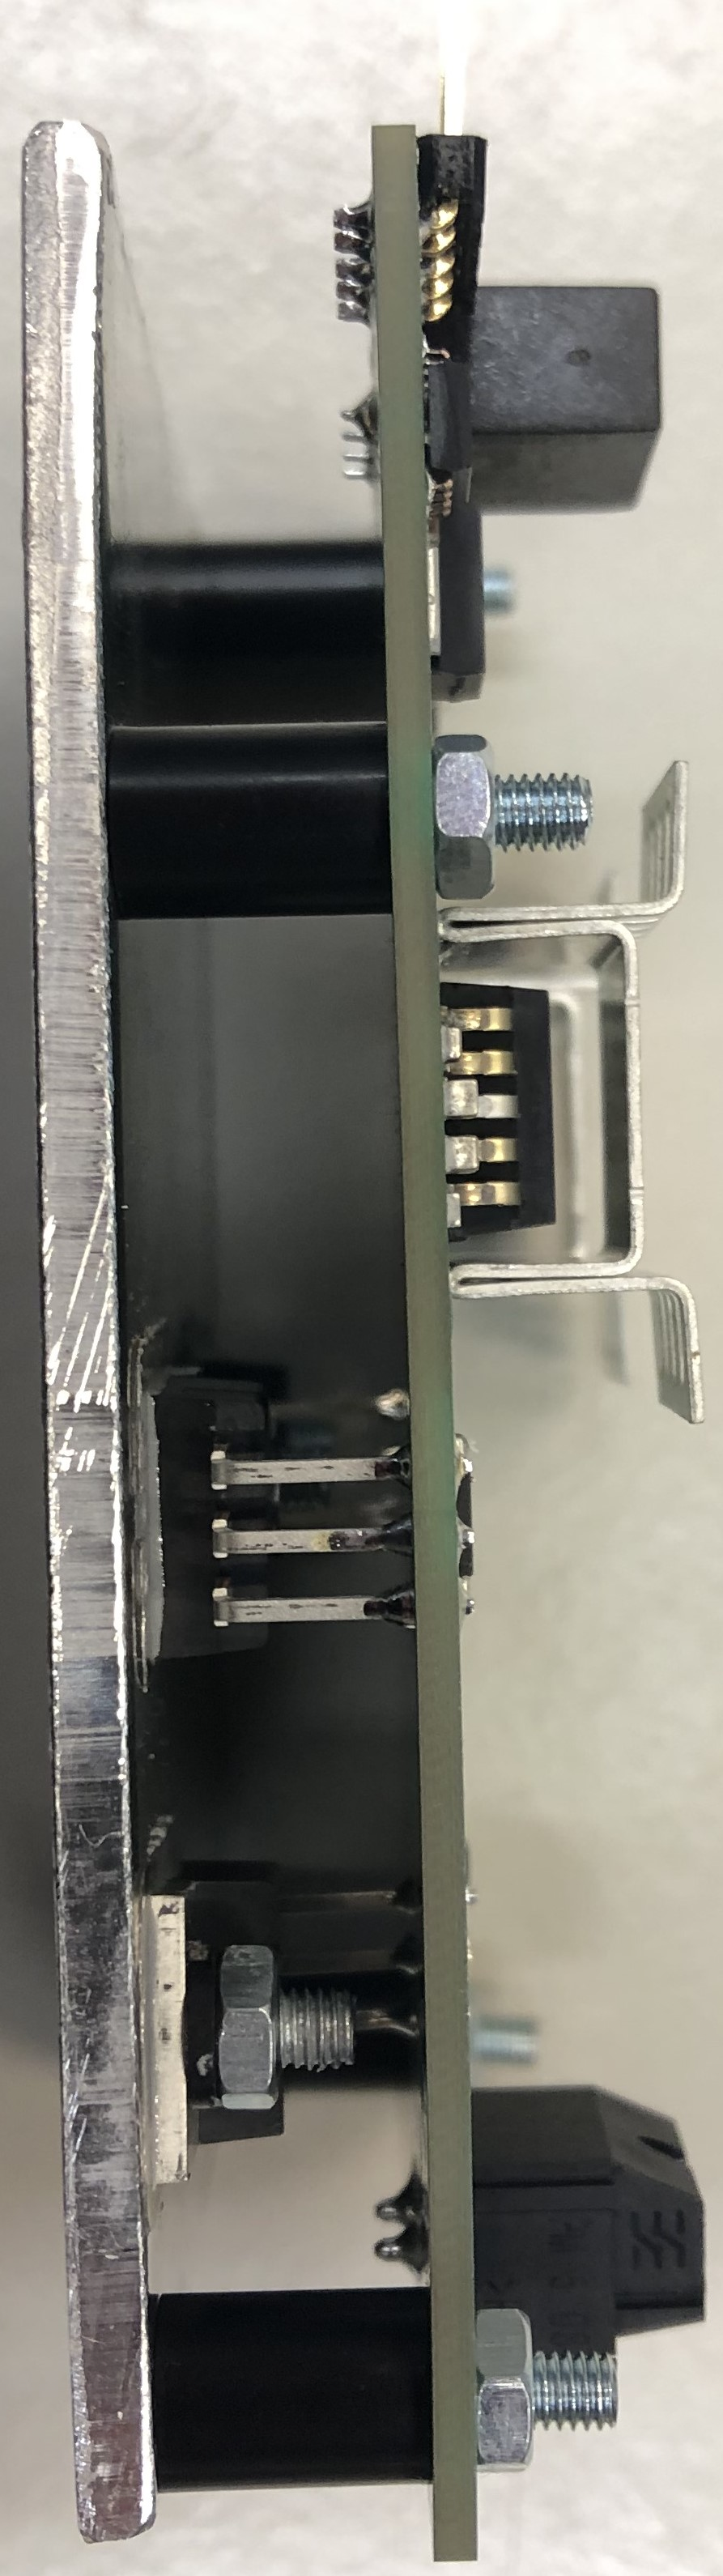
\includegraphics[scale=0.2]{CellBoardSide.jpg}
    \caption{Side view of cell board.}
    \label{fig:CellBoardSide}
\end{figure}

\begin{figure}[h!]
    \centering
    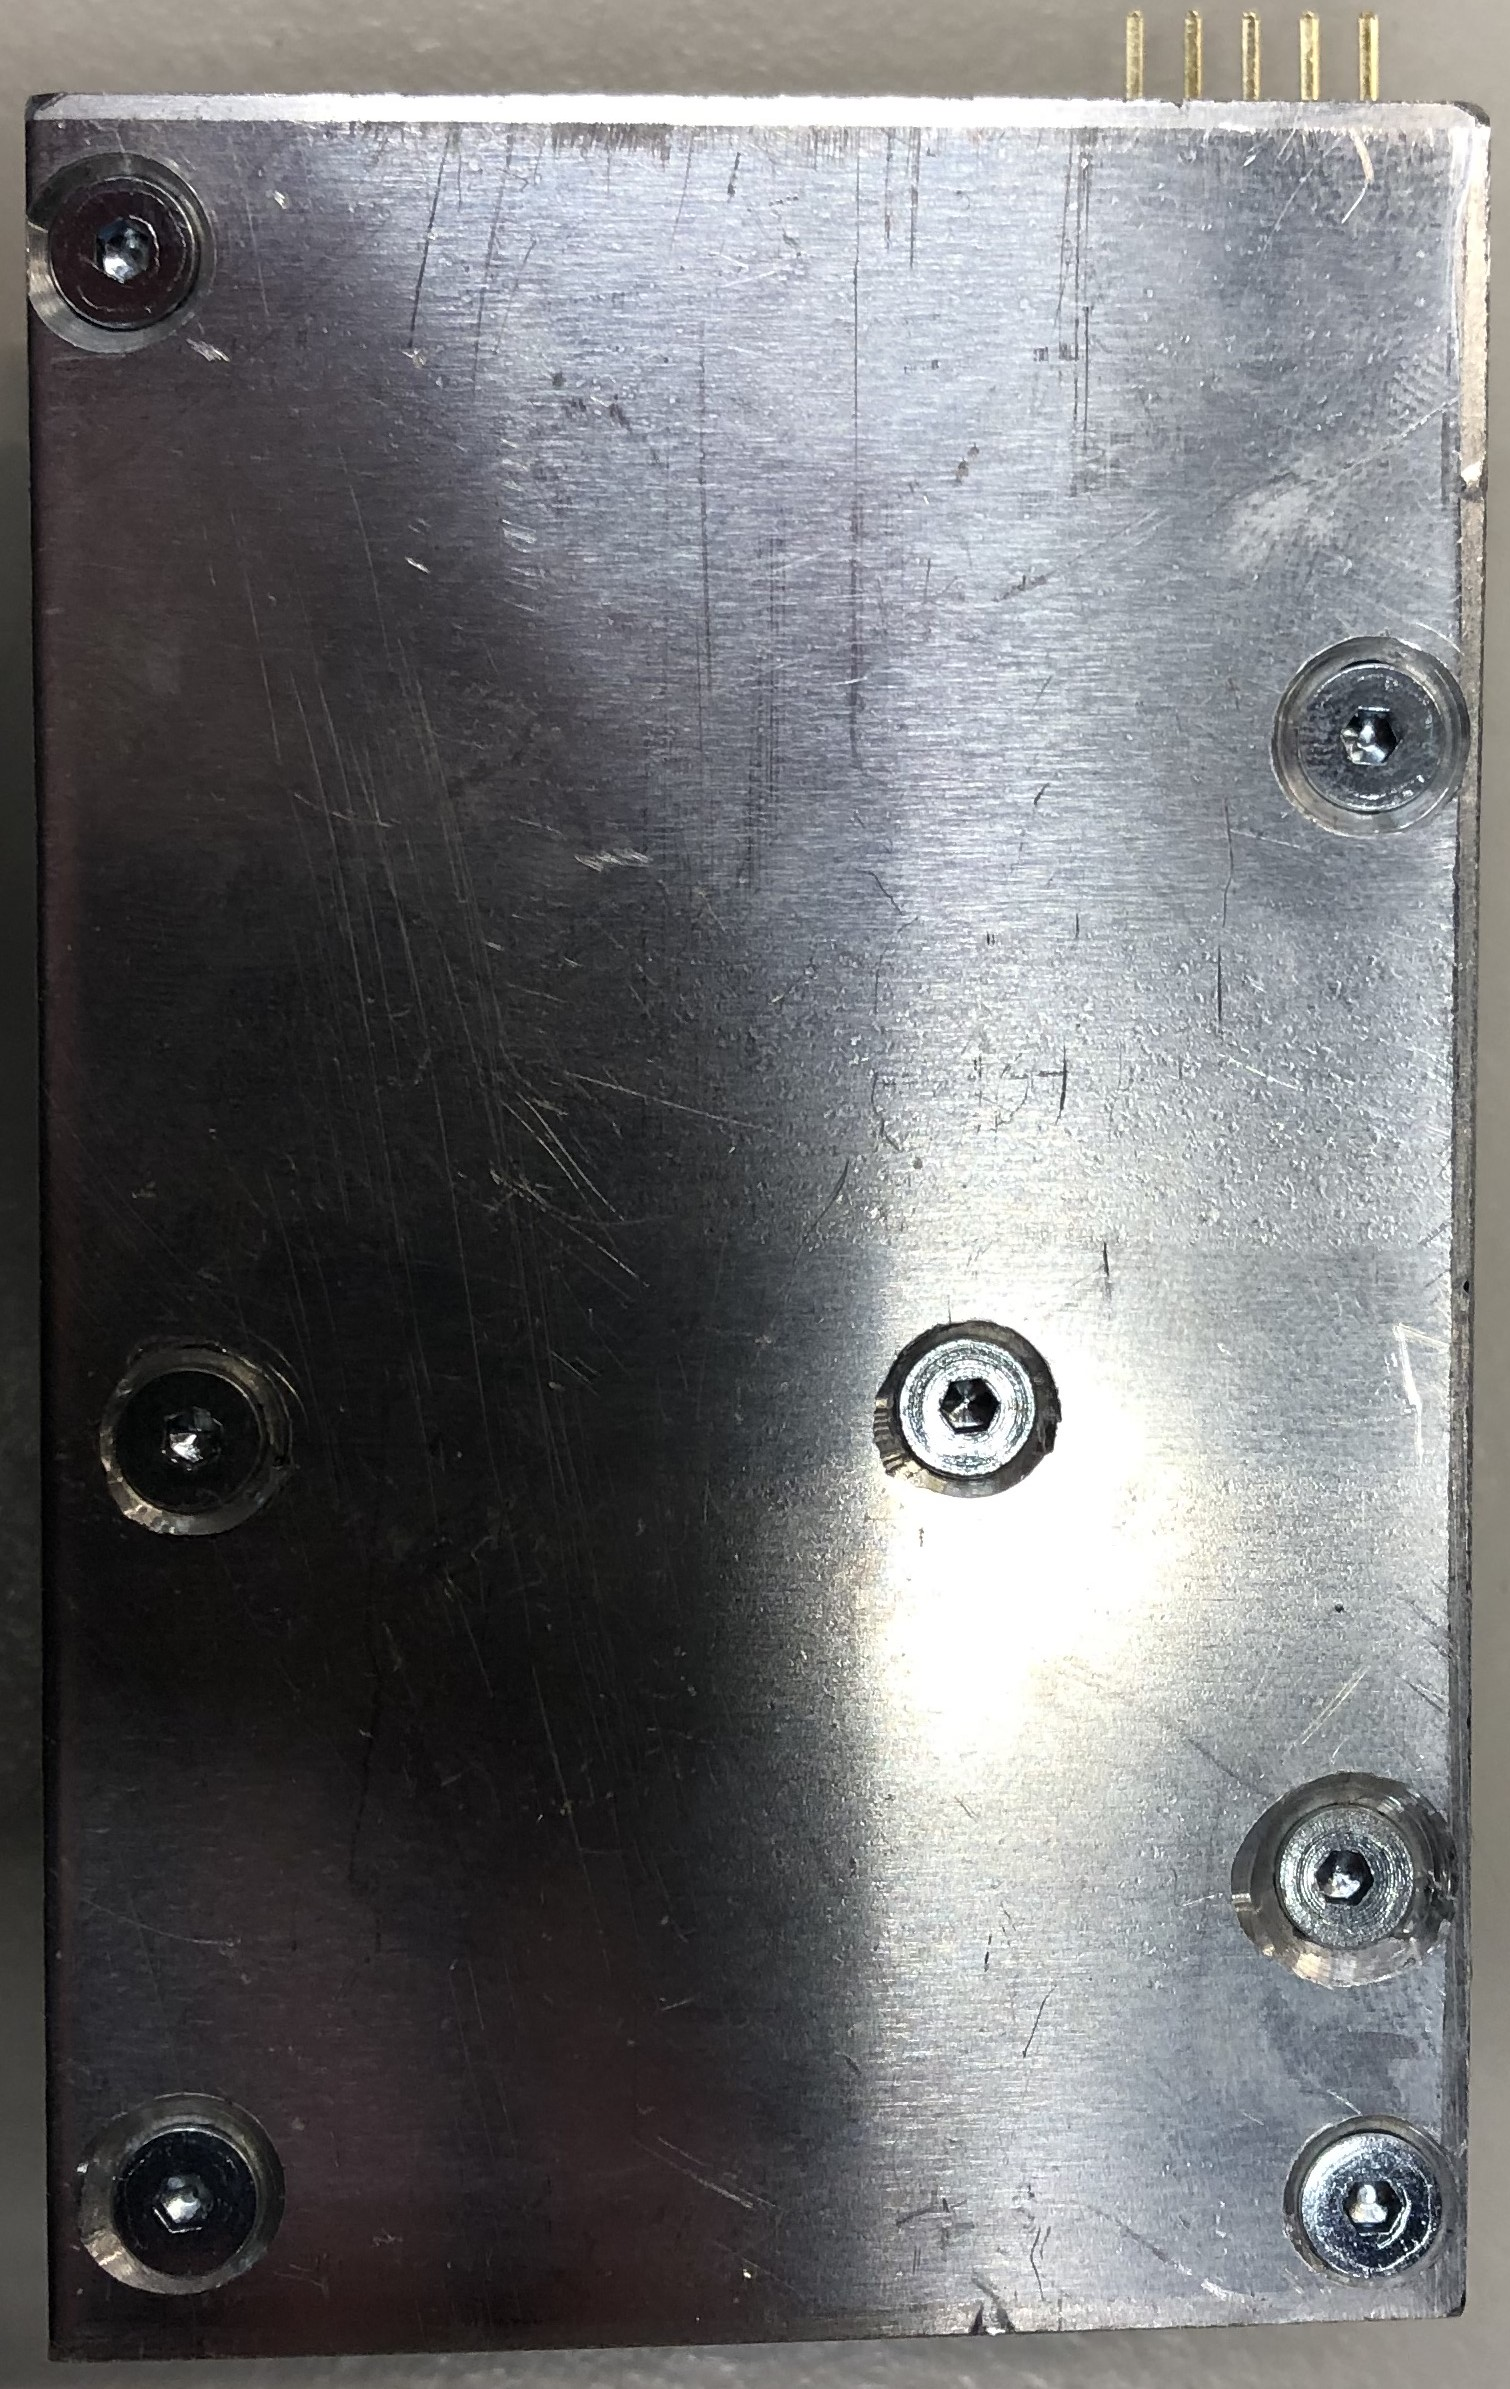
\includegraphics[scale=0.2]{CellBoardBottom.jpg}
    \caption{Bottom view of cell board.}
    \label{fig:CellBoardBottom}
\end{figure}

\begin{figure}[h!]
    \centering
    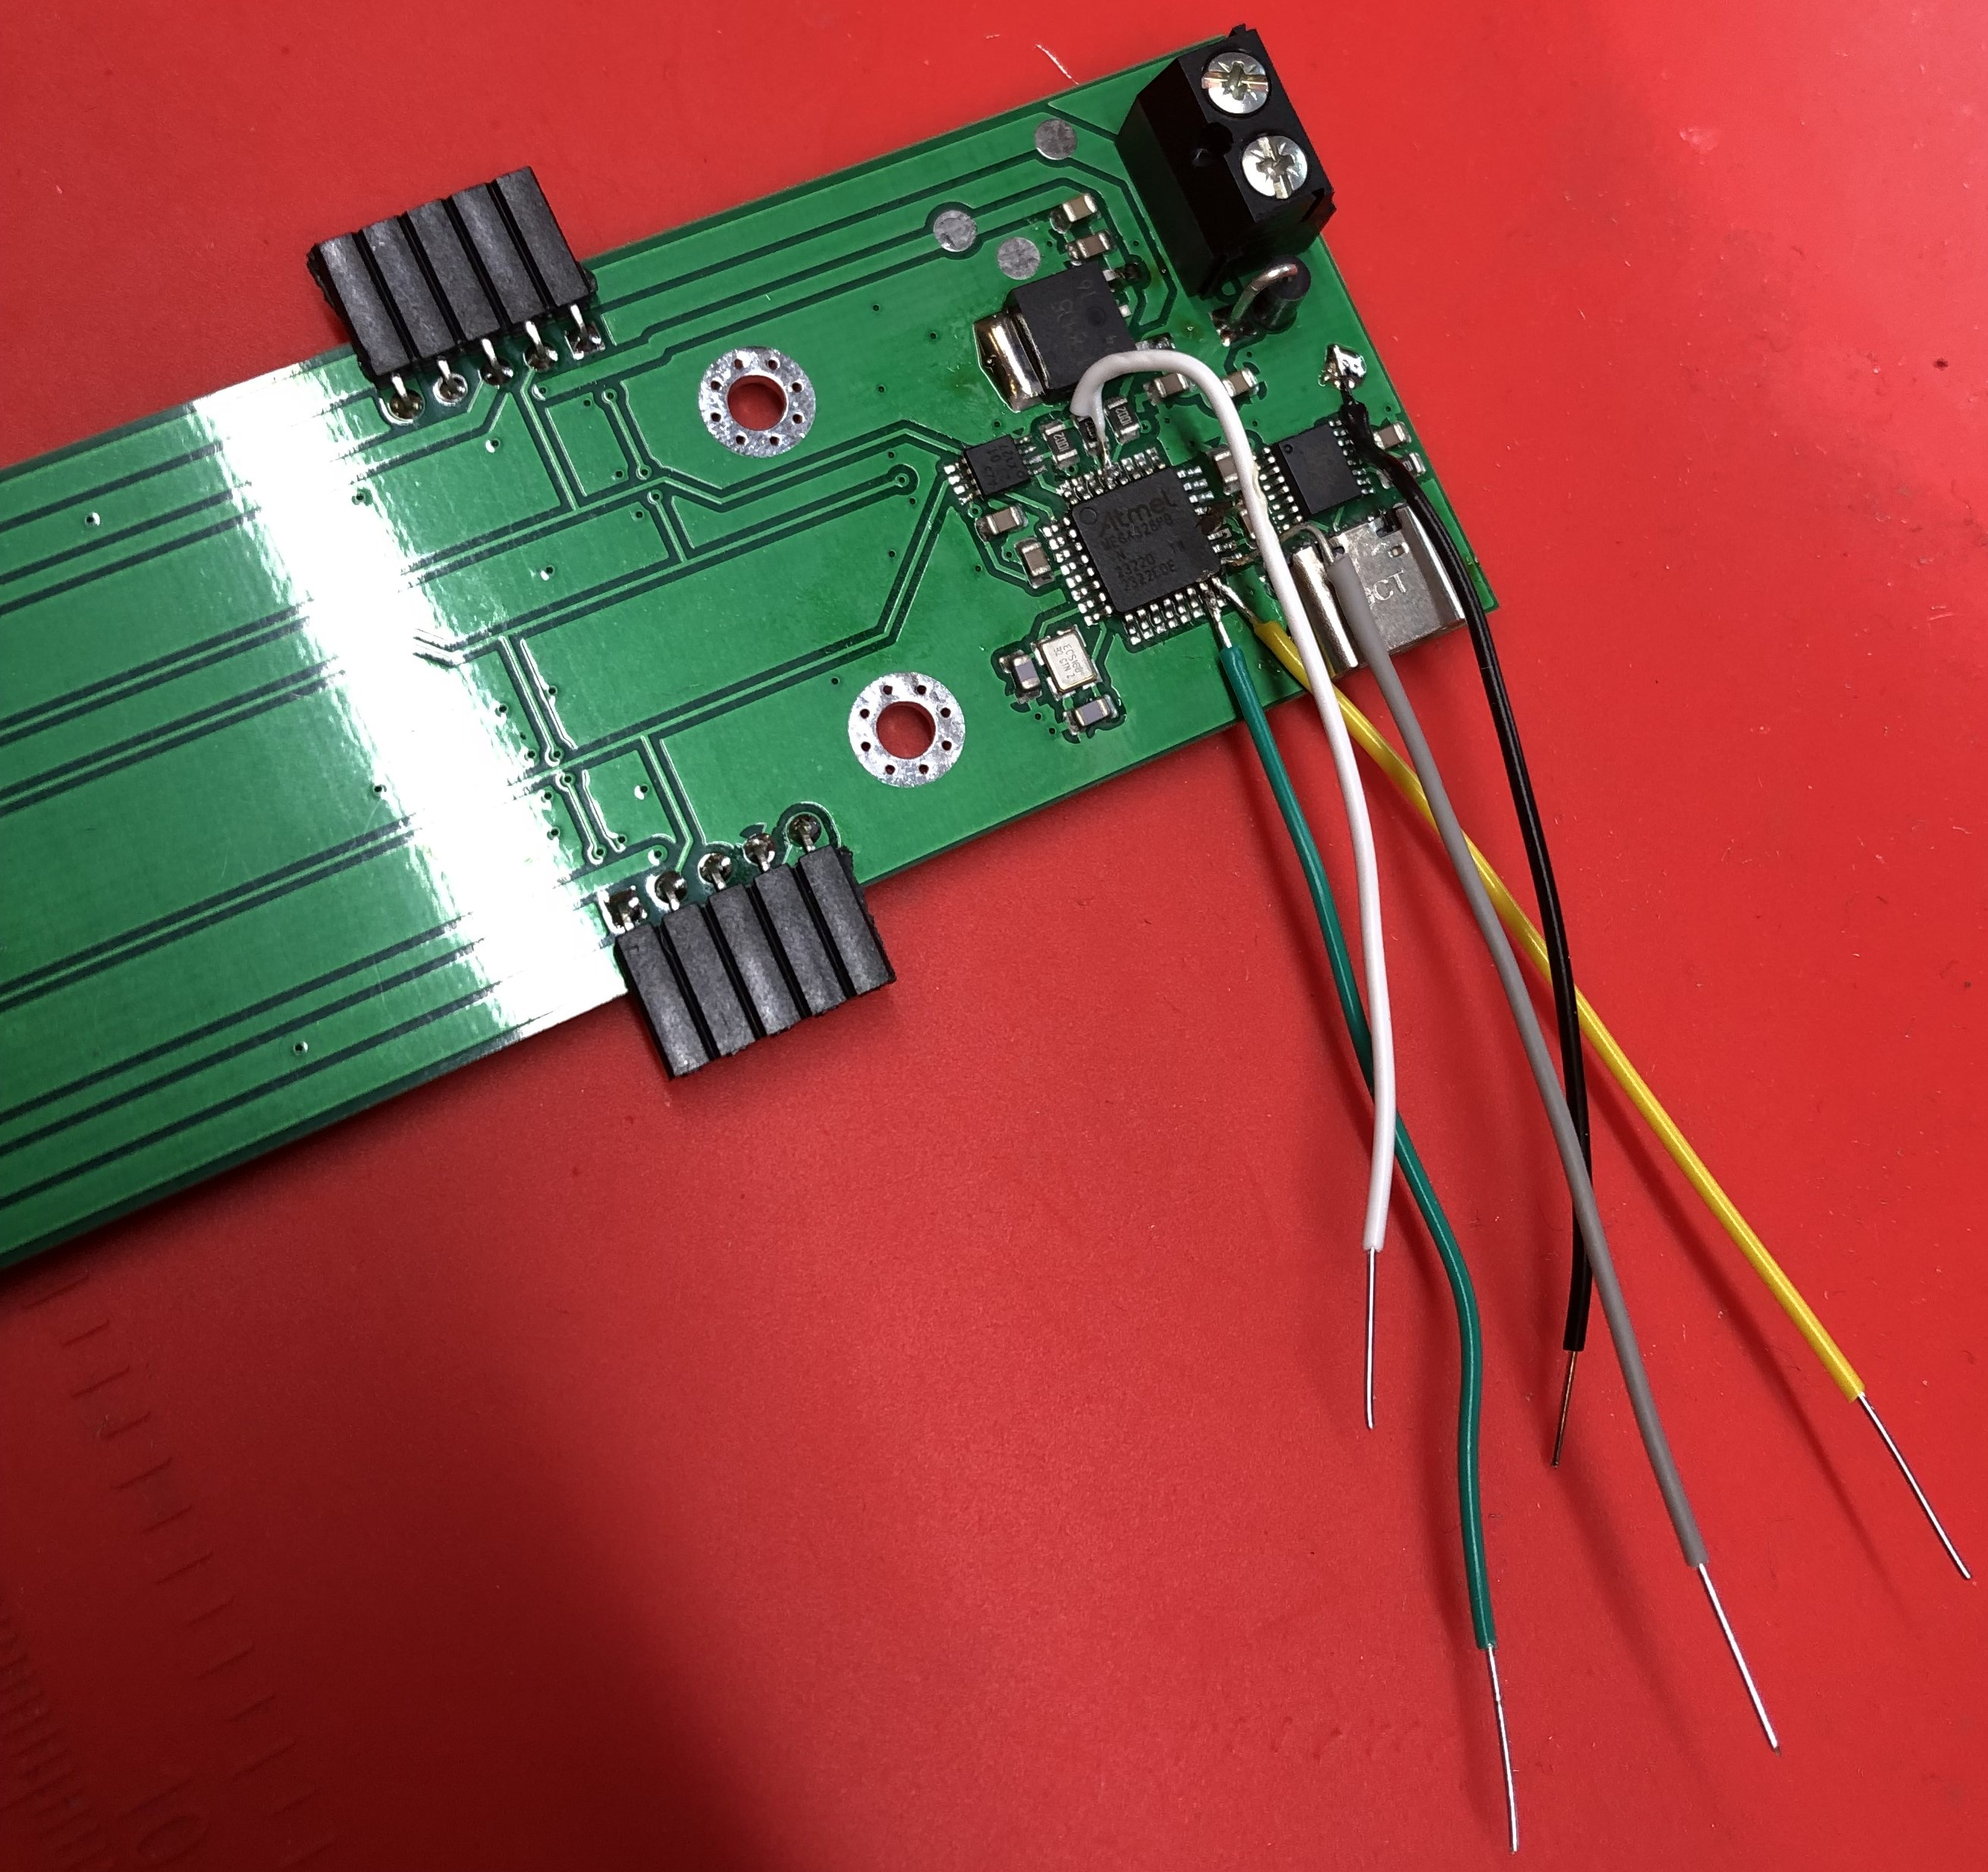
\includegraphics[scale=0.2]{ModelBoardTop.jpg}
    \caption{Top view of model board.}
    \label{fig:ModelBoardTop}
\end{figure}
\FloatBarrier